\chapter{Software}
\label{chap:software}

Om de methodes te visualiseren is een GUI ontwikkeld, deze zal in dit hoofdstuk beschreven worden. In figuur \ref{fig:FFA} is de GUI te zien. De linkerkant laat de graaf zien, en aan de rechterkant zijn controllers aanwezig om de software te bedienen. Het startpunt en eindpunt worden weergegeven door respectievelijk de kleuren groen en de kleur rood. De paden waarover een flow wordt gestuurd zijn weergegeven met de kleur blauw.
De knop 'Next flow' zal 1 augmented path zoeken met behulp van de methode die gekozen kan worden in de dropdown box. Wanneer een augmented path is gevonden zal de maximale flow voor dat pad er doorheen gestuurd worden. De knop 'Max flow' zal de actie die gedaan wordt voor de knop 'Next flow' uitvoeren tot er geen augmented path meer te vinden is. De dropdown box die zojuist genoemd is, is te vinden aan de rechterkant van de knop 'Max flow'. In deze dropdown box kan gekozen worden voor de methode die gebruikt dient te worden voor het zoeken naar een augmented path. Er kan gekozen worden tussen $DFS$ (Depth-first search), $BFS$ (Breadth-first search) en $DIJKSTRA$ (Dijkstra's algorime). De knop daarnaast, 'Reset', zal alle waardes voor de graaf weer op hun oorspronkelijke waarde zetten.
Onder de zojuist genoemde knoppen is een knop en een veld te vinden waarmee een graaf bestand geladen kan worden, deze bestanden moeten geplaatst zijn in de hoofdmap van de software. De opbouw van dit bestand zal later besproken worden. Wanneer een bestandsnaam is ingevoerd en de knop 'Load' wordt ingedrukt zal de graaf geladen worden aan de linkerkant.
Onder de knop 'Load' en het invoerveld is een veld te vinden waarin de status van de graaf weergegeven zal worden.

\begin{figure}[h]
	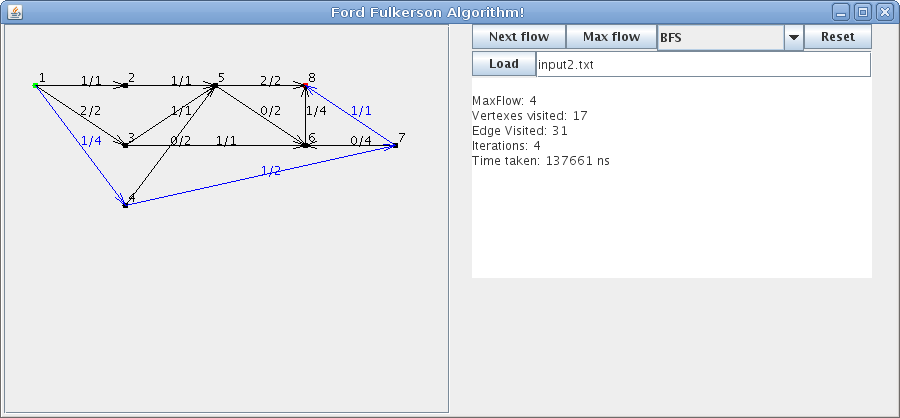
\includegraphics{software/FFA}
	\centering
	\caption{Screenshot van de GUI}
	\label{fig:FFA}
\end{figure}

Hieronder is een voorbeeld te zien van de opbouw van het bestand voor graaf 1. Op de eerste regel staan respectievelijk het aantal knopen en het aantal kanten.
Op de tweede regel staat respectievelijk het startpunt en het eindpunt.
De volgende regels bevatten de kanten van de graaf door respectievelijk de beginknoop, de eindknoop en de capaciteit van de kant te benoemen.

\begin{lstlisting}
6 8
1 6
1 2 3
1 3 3
2 3 2
2 4 3
2 6 2
3 5 2
5 6 3
4 6 2
\end{lstlisting}